\documentclass[11pt,a4paper,final]{article}

\usepackage[utf8]{inputenc}     % Codificación del archivo fuente en UTF8
\usepackage[T1]{fontenc}        % Incorpora fuente con acentos
\usepackage{amsmath}            % Amplía opciones para las ecuaciones
%\usepackage[margin=2cm]{geometry}

% -- Bibliografia --
%\usepackage[style=ieee,
%            backend=bibtex8,
%            maxcitenames=2,
%            mincitenames=1]
%            {biblatex}          % Control sobre las citas y referencias 
%  \addbibresource{Referencias.bib} % Archivo con las referencias
%\usepackage{url}                % Para incluir url clickeables

% -- Tuneando los captions --
\usepackage[margin=10pt,
            font=small,
            labelfont=bf,
            labelsep=endash]
            {caption}

% -- Tablas --
%\usepackage{booktabs}       % Decorado de tablas
%  \heavyrulewidth=1pt       % Lineas gruesas
%\usepackage{tabu}           % Permite control del ancho relativo entre columnas

% -- Figuras --
\usepackage{graphicx}		    % Permite incluir imágenes
  \graphicspath{{Figuras/}}	    % Ruta relativa donde buscar las imágenes
\usepackage[font=small,
            labelfont=bf, 
            subrefformat=parens]
            {subcaption}
            
% -- Incorporar imágenes de Matlab --
\usepackage{pgfplots}
\pgfplotsset{compat=newest} 
\pgfplotsset{plot coordinates/math parser=false}
\usepackage{tikz}
\usetikzlibrary{plotmarks} % para plotear las graficas que vienen de Matlab
            
%\usepackage{color}
%
%\sloppy
\definecolor{lightgray}{gray}{0.8} % para la grafica 2.3

%---------------------------------------------------------------------------------
% DEPRECATED COMMANDS
%---------------------------------------------------------------------------------  
\usepackage[spanish]{babel}     % Configura en modo español a muchas cosas
\usepackage{amsfonts}
\usepackage{amssymb}
\usepackage[babel,
            spanish=spanish]
            {csquotes}          % Comillas francesas en la bibliografia
%---------------------------------------------------------------------------------



\author{Sebastián R. Vanrell\\[3em]}
\title{{\large Curso:}\\\medskip
       {\Large Tópicos Selectos en Aprendizaje Maquinal}\\[3em]
       \textsf{Guía de Trabajos Prácticos Nº1}\\\bigskip
       \textsf{Algoritmos para Reconocimiento de Patrones}\\[3em]}
\date{Doctorado en Ingeniería\\\bigskip
      Facultad de Ingeniería y Ciencias Hídricas\\\bigskip
      Universidad Nacional del Litoral \\[5em]
      \today}

\usepackage{color}
\definecolor{lightgray}{gray}{0.5}
\setlength{\parindent}{0pt}

\begin{document}
\renewcommand{\tablename}{Tabla}

\maketitle
\newpage

\tableofcontents

\newpage

\section{Ejercicio 2 - Clasificación estadística de patrones}

\subsection{Ejercicio 2.1}

Sea un clasificador geométrico lineal definido por:
\begin{itemize}
\item $g_1(\mathbf{x}) = - x_1$ 
\item $g_2(\mathbf{x}) = x_1 + x_2 - 1$
\item $g_3(\mathbf{x}) = x_1 - x_2 - 1$
\end{itemize}

\begin{description}
\item[a)] Calcule y grafique las fronteras y regiones de decisión.
\end{description}

Para calcular las fronteras de decisión desarrollo las siguientes inecuaciones:
\begin{align*}
g_1(\mathbf{x}) &> g_2(\mathbf{x})   &  g_1(\mathbf{x}) &> g_3(\mathbf{x})  &  g_2(\mathbf{x}) &> g_3(\mathbf{x}) \\
- x_1           &> x_1 + x_2 - 1     &  - x_1           &> x_1 - x_2 - 1    &  x_1 + x_2 - 1   &> x_1 - x_2 - 1   \\
  x_2           &< - 2 x_1 + 1       &  x_2             &> 2 x_1 + 1        &  x_2             &> 0
\end{align*}

Para graficar las regiones de decisión (Figura \ref{ejercicio21}) considero que:
\begin{itemize}
\item $\mathbf{x} \in C_1 \;\; \mathrm{si} \;\; [g_1(\mathbf{x}) > g_2(\mathbf{x})] \wedge  [g_1(\mathbf{x}) > g_3(\mathbf{x})]$

\item $\mathbf{x} \in C_2 \;\; \mathrm{si} \;\; [g_2(\mathbf{x}) > g_1(\mathbf{x})] \wedge  [g_2(\mathbf{x}) > g_3(\mathbf{x})]$

\item $\mathbf{x} \in C_3 \;\; \mathrm{si} \;\; [g_3(\mathbf{x}) > g_1(\mathbf{x})] \wedge  [g_3(\mathbf{x}) > g_2(\mathbf{x})]$
\end{itemize}

\begin{figure}[hb]
	\centering
	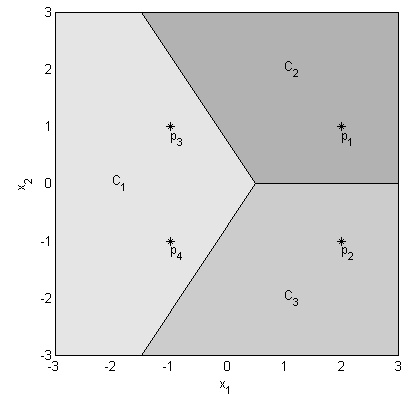
\includegraphics[width=.65\textwidth]{ejercicio21}
	\caption{Regiones y fronteras del clasificador geométrico lineal.}
	\label{ejercicio21}
\end{figure}

\begin{description}
\item[b)] Clasifique los puntos (2,1); (2,-1); (-1,1); (-1,-1).
\begin{itemize}
\item $\mathrm{p_1}:\; (2,1) \in C_2$
\item $\mathrm{p_2}:\; (2,-1) \in C_3$
\item $\mathrm{p_3}:\; (-1,1) \in C_1$
\item $\mathrm{p_4}:\; (-1,-1) \in C_1$
\end{itemize}
\end{description}



\subsection{Ejercicio 2.2}

Sean $A$ y $B$ dos clases de igual probabilidad a priori definidas por:
\begin{itemize}
\item $P(\mathbf{x}|A) \rightsquigarrow \mathcal{N}\left( 
\left(\begin{matrix}3\\0 \end{matrix}\right) ,
\left(\begin{matrix}1 & 0\\0 & 1 \end{matrix} \right) 
\right)$ 
\item $P(\mathbf{x}|B) \rightsquigarrow \mathcal{N}\left( 
\left(\begin{matrix}0\\3 \end{matrix}\right) ,
\left(\begin{matrix}1 & 0\\0 & 1 \end{matrix} \right) 
\right)$ 
\end{itemize}

\begin{description}
\item[a)] Construya un clasificador gaussiano y encuentre la frontera.
\end{description}
Dado que se pretende construir un clasificador gaussiano las funciones discriminantes son las probabilidades a posteriori:
\begin{itemize}
\item $g_A(\mathbf{x})=P(A|\mathbf{x}) = P(\mathbf{x}|A) P(A) / P(\mathbf{x})$ y
\item $g_B(\mathbf{x})=P(B|\mathbf{x}) = P(\mathbf{x}|B) P(B) / P(\mathbf{x})$.
\end{itemize} 
Como $(P(A)/P(\mathbf{x}))=(P(B)/P(\mathbf{x}))$ es un factor constante que afecta por igual a ambas funciones discriminantes se pueden simplificar a:
\begin{itemize}
\item $g_A(\mathbf{x})= P(\mathbf{x}|A) = \mathcal{N}\left( {\boldsymbol \mu}_A,{\boldsymbol\Sigma}_A \right) = \mathcal{N}\left( 
\left(\begin{matrix}3\\0 \end{matrix}\right) ,
\left(\begin{matrix}1 & 0\\0 & 1 \end{matrix} \right) 
\right)$ y
\item $g_B(\mathbf{x})= P(\mathbf{x}|B) = \mathcal{N}\left( {\boldsymbol \mu}_B,{\boldsymbol\Sigma}_B \right) = \mathcal{N}\left( 
\left(\begin{matrix}0\\3 \end{matrix}\right) ,
\left(\begin{matrix}1 & 0\\0 & 1 \end{matrix} \right) 
\right)$.
\end{itemize}
La expresión de la normal puede simplificarse aún más en este caso, sin pérdida de la capacidad discriminante de las funciones. En primer lugar se utiliza el hecho de que las matrices de covarianzas son la matriz identidad. 
\[\mathcal{N}\left( {\boldsymbol \mu},{\boldsymbol\Sigma} \right)\]
\[\mathcal{N}\left( {\boldsymbol \mu},{\boldsymbol I} \right)\]
\[\frac{1}{\sqrt{(2\pi)^2|\boldsymbol I|}}
\exp\left(-\frac{1}{2}({\mathbf x}-{\boldsymbol\mu})^T{\boldsymbol I}^{-1}({\mathbf x}-{\boldsymbol\mu})
\right)\]
\[\frac{1}{\sqrt{(2\pi)^2}}
\exp\left(-\frac{1}{2}({\mathbf x}-{\boldsymbol\mu})^T({\mathbf x}-{\boldsymbol\mu})
\right)\]
En segundo lugar, el factor que afecta a la exponencial es el mismo en ambas funciones y puede eliminarse. 
\[\exp\left(-\frac{1}{2}({\mathbf x}-{\boldsymbol\mu})^T({\mathbf x}-{\boldsymbol\mu})\right)\]
\[\exp\left(-\frac{1}{2}\parallel{\mathbf x}-{\boldsymbol\mu}\parallel^2
\right)\]
En último lugar se aplica el logaritmo natural, función que no altera las regiones de decisión, y se quita el factor constante 1/2.
\[-\frac{1}{2}\parallel{\mathbf x}-{\boldsymbol\mu}\parallel^2\]
\[-\parallel{\mathbf x}-{\boldsymbol\mu}\parallel^2 \]
Entonces las funciones discriminantes resultan ser:
\begin{itemize}
\item $g_A(\mathbf{x})= -\parallel{\mathbf x}-{\boldsymbol\mu}_A\parallel^2$ y
\item $g_B(\mathbf{x})= -\parallel{\mathbf x}-{\boldsymbol\mu}_B\parallel^2$,
\end{itemize}
donde el máximo entre ambas funciones indica la pertenencia a $A$ o $B$.

Para encontrar la frontera de decisión igualo ambas funciones:
\begin{align*}
g_A(\mathbf{x}) &= g_B(\mathbf{x}) \\
-\parallel{\mathbf x}-{\boldsymbol\mu}_A\parallel^2 &= -\parallel{\mathbf x}-{\boldsymbol\mu}_B\parallel^2 \\
\parallel{\mathbf x}-{\boldsymbol\mu}_A\parallel^2 &= \parallel{\mathbf x}-{\boldsymbol\mu}_B\parallel^2 \\
(x_1 - 3)^2 + x_2^2 &= x_1^2 +(x_2 - 3)^2\\
x_1^2 - 6 x_1 + 9 + x_2^2 &= x_1^2 + x_2^2 - 6 x_2 + 9\\
x_1 &= x_2 
\end{align*}

\begin{description}
\item[b)] Realice una representación gráfica del problema.
\end{description}
En la Figura \ref{ejercicio22} se muestra claramente la frontera de decisión (la recta) y la etiqueta de cada región. Las curvas representan las curvas de nivel de la función discriminante ganadora en cada región, a medida que se alejan de la recta van creciendo en valor.  

\begin{figure}[h]
	\centering
	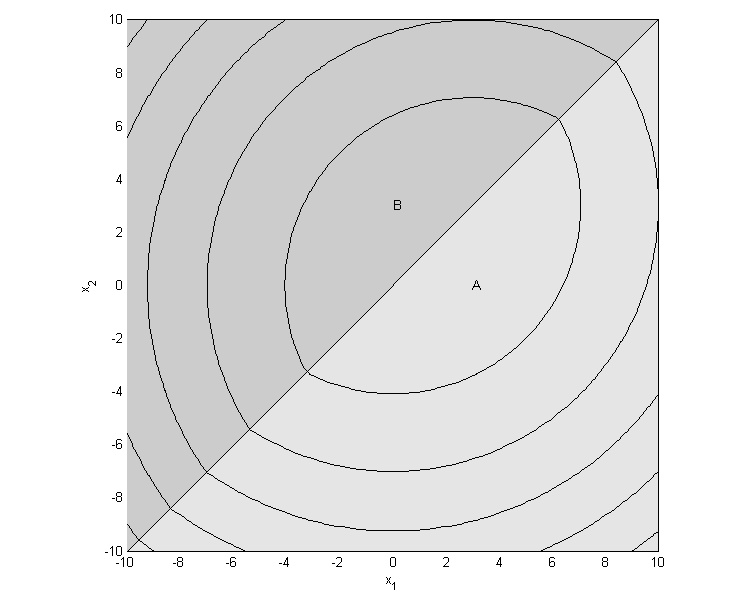
\includegraphics[scale= .5]{ejercicio22}
	\caption{Regiones y fronteras del clasificador gaussiano.}
	\label{ejercicio22}
\end{figure}


\clearpage


\subsection{Ejercicio 2.3}

Implemente un clasificador gaussiano por ML para el mini-corpus de muestras proporcionado, realizando una representación gráfica de la situación:

\begin{description}
\item[a)] Clasifique los datos del conjunto de entrenamiento y calcule la tasa de aciertos.

\item[b)] A partir de los parámetros obtenidos genere nuevos datos de prueba, clasifíquelos y compare con el resultado anterior.
\end{description}

\begin{verbatim}
% Cargo los datos (patrones con sus clases respectivas)
data = load('gaussDATA.txt', '-ascii'); % cargo los datos
x = data(:,1:2); % patrones
c = data(:,3);   % identificador de clase
N = length(c);   % cantidad de ejemplos

c1 = find(c== 1); % indices de clase 1
c2 = find(c== 2); % indices de clase 2
c3 = find(c== 3); % indices de clase 3
c4 = find(c== 4); % indices de clase 4

hold on
plot(x(c1,1), x(c1,2), 'ok')
plot(x(c2,1), x(c2,2), 'xk')
plot(x(c3,1), x(c3,2), 'dk')
plot(x(c4,1), x(c4,2), 'sk')
hold off

xlabel('x_1'); ylabel('x_2');
legend('clase 1','clase 2','clase 3','clase 4')
title('Distribución de los patrones separados por clase')
\end{verbatim}

\begin{figure}
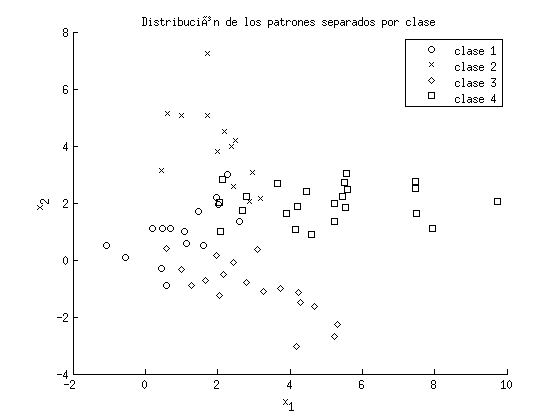
\includegraphics [width=0.9\textwidth]{Ejercicio2_01.png}
\caption{Distribución de los patrones del mini-corpus indicando la clase de cada uno.}
\label{fig:ejercicio231}
\end{figure}


Por la gráfica de la Figura \ref{fig:ejercicio231} se deduce que deberán utilizarse gaussianas con media desconocida y covarianza no isotrópica desconocida. Separo los patrones de entrenamiento para estimar las medias y matrices de covarianzas de cada clase.

\begin{verbatim}
% Divido los patrones a utilizar en el entrenamiento de los de testeo
nentre = floor(0.8 * N); % 80% de los patrones para entrenamiento
ntest = N - nentre;      % 20% de los patrones para testeo
ientre = randperm(N,nentre); % indices utilizados en el entrenamiento
itest = setdiff(1:N,ientre); % indices utilizados para el testeo

% Estimación de los parámetros para cada clase, con los patrones de
% entrenamiento
% medias estimadas
u1 = mean(x(intersect(c1,ientre),:));
u2 = mean(x(intersect(c2,ientre),:));
u3 = mean(x(intersect(c3,ientre),:));
u4 = mean(x(intersect(c4,ientre),:));
% matrices de covarianzas estimadas
sig1 = cov(x(intersect(c1,ientre),:));
sig2 = cov(x(intersect(c2,ientre),:));
sig3 = cov(x(intersect(c3,ientre),:));
sig4 = cov(x(intersect(c4,ientre),:));

% clasifico los patrones de entrenamiento
centre = zeros(size(c)); % clases asignadas durante el entrenamiento
for n = ientre
    xn = x(n,:); % voy leyendo de a un dato

    % Calculo los valores de las funciones discriminantes para xn
    g1 = mvnpdf(xn, u1, sig1);
    g2 = mvnpdf(xn, u2, sig2);
    g3 = mvnpdf(xn, u3, sig3);
    g4 = mvnpdf(xn, u4, sig4);

    % Busco cual es la clase ganadora, asigno 0 si cae en la frontera
    if     g1 > max([g2 g3 g4])
        centre(n) = 1;
    elseif g2 > max([g1 g3 g4])
        centre(n) = 2;
    elseif g3 > max([g1 g2 g4])
        centre(n) = 3;
    elseif g4 > max([g1 g2 g3])
        centre(n) = 4;
    else
        centre(n) = 0;
    end
end

% busco cuales patrones fueron confundidos al clasificar
cmal = intersect(find(c~=centre), ientre); % patrones mal identificados
cbien = setdiff(ientre,cmal); % patrones identificados correctamente

fprintf('La tasa de aciertos en el entrenamiento es de %0.2f %%\n', ...
        100*length(cbien)/nentre);
% disp(['La tasa de aciertos es de ' num2str(100*nnz(cright)/N) '%'])

hold on; plot(x(cmal,1), x(cmal,2), '.r'); hold off
\end{verbatim}

%\begin{figure}[h]
%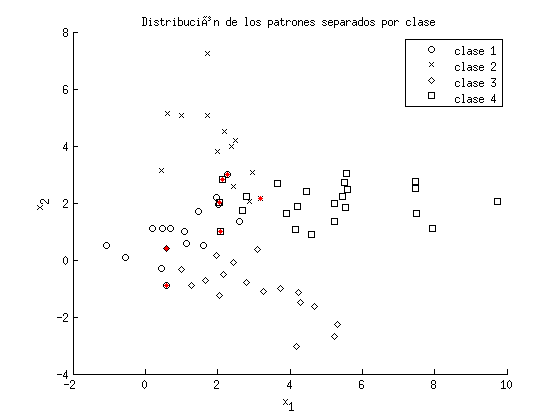
\includegraphics [width=0.9\textwidth]{Ejercicio2_02.png}
%\caption{Los patrones indicados con puntos rojos fueron clasificados incorrectamente durante el entrenamiento.}
%\label{fig:ejercicio232}
%\end{figure}

En el entrenamiento se utilizaron el 80\% de los patrones de la Figura \ref{fig:ejercicio233}. Aquellos indicados con puntos rojos fueron clasificados incorrectamente durante el entrenamiento. Considerando sólo los patrones de entrenamiento se obtuvo el siguiente reporte:

\color{lightgray} \begin{verbatim}La tasa de aciertos en el entrenamiento es de 87.27 %
\end{verbatim} \color{black}

Ahora se clasifican los patrones para testeo y se calcula la tasa de reconocimiento.

\begin{verbatim}
% clasifico los patrones de testeo
% --------------------------------
ctest = zeros(size(c)); % clases asignadas durante el testeo
for n = itest
    xn = x(n,:); % voy leyendo de a un dato

    % Calculo los valores de las funciones discriminantes para xn
    g1 = mvnpdf(xn, u1, sig1);
    g2 = mvnpdf(xn, u2, sig2);
    g3 = mvnpdf(xn, u3, sig3);
    g4 = mvnpdf(xn, u4, sig4);

    % Busco cual es la clase ganadora, asigno 0 si cae en la frontera
    if     g1 > max([g2 g3 g4])
        ctest(n) = 1;
    elseif g2 > max([g1 g3 g4])
        ctest(n) = 2;
    elseif g3 > max([g1 g2 g4])
        ctest(n) = 3;
    elseif g4 > max([g1 g2 g3])
        ctest(n) = 4;
    else
        ctest(n) = 0;
    end
end

% busco cuales patrones fueron confundidos al clasificar
cmal = intersect(find(c~=ctest), itest); % patrones mal identificados
cbien = setdiff(itest,cmal); % patrones identificados correctamente

fprintf('La tasa de aciertos en el testeo es de %0.2f %%\n', ...
        100*length(cbien)/ntest);

hold on; plot(x(cmal,1), x(cmal,2), '*b'); hold off
\end{verbatim}

\begin{figure}[h]
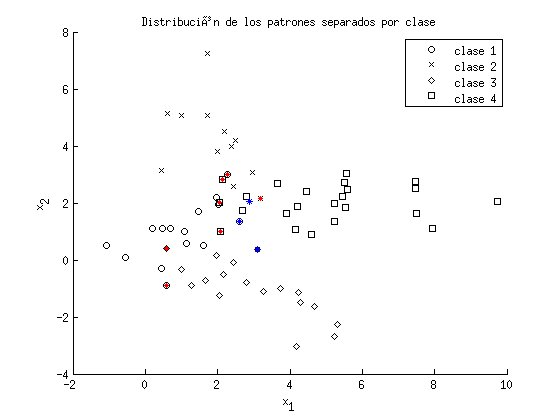
\includegraphics [width=0.9\textwidth]{Ejercicio2_03.png}
\caption{Los patrones indicados con puntos rojos fueron clasificados incorrectamente durante el entrenamiento, y los indicados con asteriscos azules durante el testeo.}
\label{fig:ejercicio233}
\end{figure}

En el testeo se utilizaron el 20\% restante de los patrones de la Figura \ref{fig:ejercicio233}. Los indicados con asteriscos azules fueron clasificados incorrectamente. Luego del testeo se obtuvo el siguiente reporte:

\color{lightgray} \begin{verbatim}La tasa de aciertos en el testeo es de 78.57 %
\end{verbatim} \color{black}
    
Por último se realizó una gráfica (Figura \ref{fig:ejercicio234}) representativa de las regiones definidas durante el entrenamiento.

\begin{verbatim}
T = 100;
x1 = linspace(-2,10,T);
x2 = linspace(-4,8,T);
[X1,X2] = meshgrid(x1,x2);
for i = 1:T
    for j = 1:T
        xn = [x1(i) x2(j)];
        gc1(i,j) = mvnpdf(xn, u1, sig1);
        gc2(i,j) = mvnpdf(xn, u2, sig2);
        gc3(i,j) = mvnpdf(xn, u3, sig3);
        gc4(i,j) = mvnpdf(xn, u4, sig4);
    end
end

gc1234 = cat(3, gc1, gc2, gc3, gc4);

[maxg, maxc] = max(gc1234,[],3);

figure
grises = linspace(0.7,0.9,64);
colormap(repmat(grises',1,3))
surf(X1,X2,maxc'-4,'EdgeColor','none')
hold on; contour(X1,X2,maxg',5,'k'); hold off;
view(2); axis square
xlabel('x_1'); ylabel('x_2');
title('Regiones de decisión')

text([u1(1) u2(1) u3(1) u4(1)], [u1(2) u2(2) u3(2) u4(2)],...
    {'C_1','C_2','C_3','C_4'})
\end{verbatim}

\begin{figure}[h]
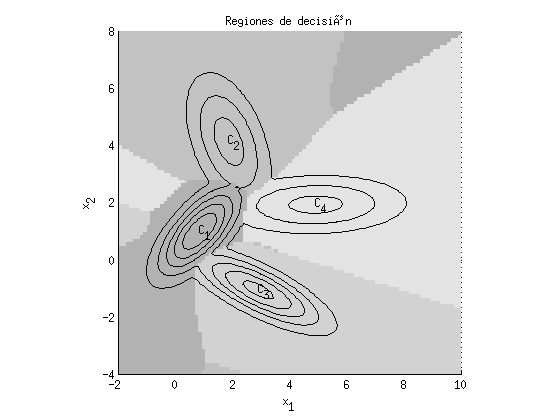
\includegraphics [width=0.9\textwidth]{Ejercicio2_04.png}
\caption{Regiones de decisión utilizadas para clasificar. Las curvas de nivel corresponden a las funciones discriminantes en cada región.}
\label{fig:ejercicio234}
\end{figure}


\clearpage







\section{Ejercicio 3 - Análisis estadístico de datos - PCA}



\subsection{Ejercicio 3.1}


Implemente el algoritmo de PCA.


Debajo se copia el código fuente de la función implementada. La descripción de la misma se encuentra dentro del código.

\subsubsection*{mipca.m}

\begin{verbatim}
1     function [PC, autoval] = mipca( X )
2     %MIPCA devuelve la matriz que permite proyectar los datos X sobre las
3     %direcciones obtenidas por medio del análisis de componentes principales.
4     % X es una matriz de D por N, donde cada observación se acomoda como
5     % columna. D es la dimensión de cada observación y N es el
6     % número total de observaciones.
7     %
8     % PC es la matriz de transformación de la base original a las direcciones
9     % principales. Las columnas son los versores de la nueva base.
10    %
11    % autoval es un vector con los autovalores asociados a PC, en orden 
12    % decreciente.
13    
14    % Matriz de covarianza (internamente realiza la resta de la media)
15    S = cov(X'); % traspongo para que tome bien las observaciones
16    
17    % Obtengo la matriz de autovectores y una matriz con los autovalores de S
18    [autovec, autoval] = eig(S);
19    
20    % Ordeno la matriz de transformación por orden descendente de autovalores
21    PC = fliplr(autovec);
22    
23    % Autovalores ordenados por módulo decreciente
24    autoval = flipdim(diag(autoval),1);
25    
26    end
\end{verbatim}
    

\subsection{Ejercicio 3.2}


Escriba un programa que le permita generar datos aleatorios $\mathbf(x)$ a partir del siguiente modelo generativo lineal: $\mathbf(x) = \mathbf(A) \mathbf(s)$, donde $\mathbf(s)$ es el vector de fuentes (aleatorio) y $\mathbf(A)$ es la matriz de mezcla.

Debajo se copia el código fuente de la función implementada. La descripción de la misma se encuentra dentro del código.

\subsubsection*{mezclar.m}
\begin{verbatim}
1     function X = mezclar( A, s1, s2 )
2     %MEZCLAR X = ( A, s1, s2 ) dada la matriz de mecla A y las fuentes s1 y s2 
3     % (vectores) se generan dos mezclas x1 y x2 (cada una en un renglón de X).
4     
5     if size(s1,1) ~= 1
6         s1 = s1'; % convierte s1 en un vector horizontal si no lo es
7     end
8     if size(s2,1) ~= 1
9         s2 = s2'; % convierte s2 en un vector horizontal si no lo es
10    end
11    
12    S = vertcat(s1,s2);
13    X = A * S;
14    end
\end{verbatim}
    

\subsection{Ejercicio 3.3}

A partir de datos de dos mezclas, obtenidos mediante dos fuentes y una matriz de mezcla aleatoria, utilice PCA para lo siguiente:

\begin{enumerate}
   \item[a)] Pruebe con fuentes con distribución gaussiana y laplaciana, para matrices de mezcla con columnas ortogonales y no ortogonales.
   \item[b)] Para cada caso de los anteriores y cada etapa (fuentes, mezclas, señales separadas) dibuje un gráfico de dispersión de las variables.
   \item[c)] Luego de la separación obtenga la matriz $\mathbf{W}$ correspondiente.
\end{enumerate}
\begin{verbatim}
N = 300;

% Fuentes gaussianas y laplacianas
s{1} = randgauss1D(1, 1, N)';
s{2} = randgauss1D(3, 3, N)';
s{3} = randlap(N, 2 ,2)';
s{4} = randlap(N, 5 ,0.9)';
s{5} = randgauss1D(1, 1, N)';
s{6} = randlap(N, 2 ,2)';

% Se corroboran los signos para impedir que ambas mezclas sean
% proporcionales
signos = ones(2);
while isequal(signos(1,:),signos(2,:)) || isequal(signos(1,:), -signos(2,:))
    signos = sign(rand(2)-0.5);
end

% Generacion aleatoria de las matrices de mezcla
A{1} = repmat(2*rand(1,2)-1,2,1) .* signos;% Mezcla con columnas ortogonales
A{2} = (2*rand(2)-1) .* signos;            % Mezcla no ortogonal
titort{1} = 'ortogonales';
titort{2} = 'no ortogonales';
suptit{1} = 'Fuentes gaussianas';
suptit{2} = 'Fuentes laplacianas';
suptit{3} = 'Fuente gaussiana y laplaciana';

for ss = 1:3
    figure
    for aa = 1:2
        X = mezclar(A{aa},s{2*ss-1},s{2*ss}); % Mezcla las señales
        x1m = mean(X(1,:)); % media de la primera dimension
        x2m = mean(X(2,:)); % media de la segunda dimension

        W = mipca(X); % Obtengo la Matriz de Proyección de X sobre las
                      % direcciones principales, versores por columnas

        Y = W' * X; % Proyecto los datos sobre las direcciones principales
        % y_1  = w_11 * x_1 + w_21 * x_2
        % y_2  = w_12 * x_2 + w_22 * x_2

        subplot(2,3,1+3*(aa-1))
        scatter(s{2*ss-1}, s{2*ss}); axis equal;
        title({'Fuentes';['columnas ' titort{aa}]} )
        xlabel('s_1'); ylabel('s_2');

        subplot(2,3,2+3*(aa-1))
        scatter(X(1,:), X(2,:)); axis equal;
        hold on;
        plot(x1m + [0 5*W(1,1)],x2m + [0 5*W(2,1)], 'k','LineWidth',2)
        plot(x1m + [0 5*W(1,2)],x2m + [0 5*W(2,2)], 'k','LineWidth',2)
        hold off
        title({'Mezclas';['columnas ' titort{aa}]} )
        xlabel('x_1'); ylabel('x_2');

        subplot(2,3,3+3*(aa-1))
        scatter(Y(1,:), Y(2,:)); axis equal;
        title({'Señales separadas';['columnas ' titort{aa}]} )
        xlabel('y_1'); ylabel('y_2');

        Ainv  = inv(A{aa});
        disp([suptit{ss} ', columnas ' titort{aa}])
        fprintf(['A = [%0.2f %0.2f],\t Ainv = [%0.2f %0.2f],\t W = [%0.2f %0.2f]\n'...
                 '    [%0.2f %0.2f],\t Ainv = [%0.2f %0.2f],\t     [%0.2f %0.2f]\n\n'],...
                 A{aa}(1,:), Ainv(2,:), W(1,:), A{aa}(2,:), Ainv(2,:), W(2,:) );
    end
    suptitle(suptit{ss})
end
\end{verbatim}


En las Figuras \ref{fig:ejercicio331}, \ref{fig:ejercicio332} y \ref{fig:ejercicio333} se muestra cada una de las etapas requeridas. En las gráficas de las mezclas se dibujan las direcciones principales identificadas mediante PCA. La fila superior corresponde a matrices de mezclas con columnas ortogonales, la inferior a columnas no ortogonales.

Las matrices de mezcla y separación utilizadas se listan a continuación, para cada caso:
\begin{verbatim}Fuentes gaussianas, columnas ortogonales
A = [0.94 -0.74],	 Ainv = [0.53 0.53],	 W = [-0.71 -0.70]
    [0.94 0.74],	        [-0.67 0.67],	     [0.70 -0.71]

Fuentes gaussianas, columnas no ortogonales
A = [-0.05 0.54],	 Ainv = [0.15 -1.22],	 W = [-0.98 0.21]
    [-0.82 0.07],	        [1.86 -0.11],	     [-0.21 -0.98]

Fuentes laplacianas, columnas ortogonales
A = [0.94 -0.74],	 Ainv = [0.53 0.53],	 W = [0.70 -0.72]
    [0.94 0.74],	        [-0.67 0.67],	     [0.72 0.70]

Fuentes laplacianas, columnas no ortogonales
A = [-0.05 0.54],	 Ainv = [0.15 -1.22],	 W = [0.06 -1.00]
    [-0.82 0.07],	        [1.86 -0.11],	     [1.00 0.06]

Fuente gaussiana y laplaciana, columnas ortogonales
A = [0.94 -0.74],	 Ainv = [0.53 0.53],	 W = [-0.66 -0.75]
    [0.94 0.74],	        [-0.67 0.67],	     [0.75 -0.66]

Fuente gaussiana y laplaciana, columnas no ortogonales
A = [-0.05 0.54],	 Ainv = [0.15 -1.22],	 W = [-0.99 0.12]
    [-0.82 0.07],	        [1.86 -0.11],	     [-0.12 -0.99]
\end{verbatim}

\begin{figure}
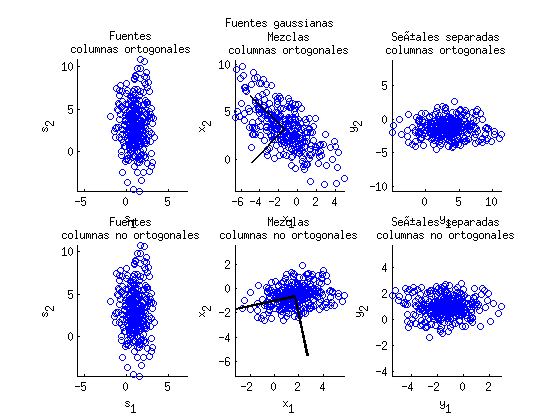
\includegraphics [width=\textwidth]{Ejercicio3_01.png}
\caption{PCA aplicado a fuentes gaussianas.}
\label{fig:ejercicio331}
\end{figure}
\begin{figure}
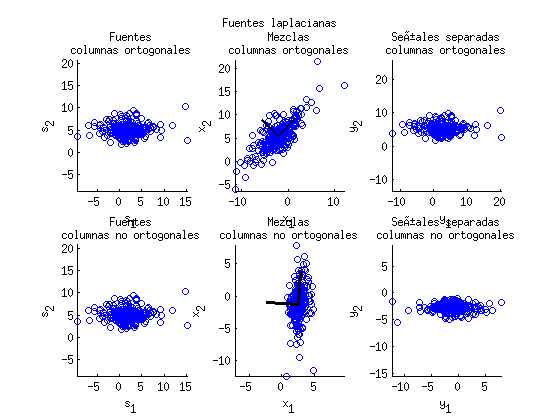
\includegraphics [width=\textwidth]{Ejercicio3_02.png}
\caption{PCA aplicado a fuentes laplacianas.}
\label{fig:ejercicio332}
\end{figure}
\begin{figure}
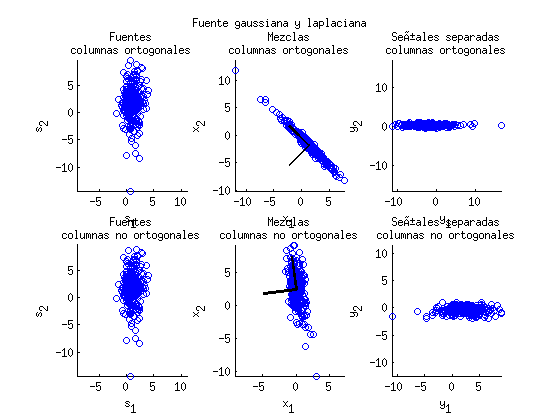
\includegraphics [width=\textwidth]{Ejercicio3_03.png}
\caption{PCA aplicado a una fuente gaussiana y otra laplaciana.}
\label{fig:ejercicio333}
\end{figure}


\begin{enumerate}
   \item[d)] ¿La matriz de separación $\mathbf{W}$ es la inversa de la matriz de mezcla $\mathbf{A}$ utilizada?
\end{enumerate}

Para responder a la pregunta desarrollo la siguiente expresión:

$\mathbf{y} = \mathbf{W} \mathbf{x} = \mathbf{W} \mathbf{A} \mathbf{s}$

Si la matriz de separación $\mathbf{W}$ fuera la inversa de la matriz de mezcla $\mathbf{A}$ entonces utilizando PCA se podría recuperar las fuentes. Sin embargo, en las pruebas anteriores no se corrobora que $\mathbf{W}$ sea la inversa de $\mathbf{A}$. Al proyectar sobre las direcciones principales se provoca una rotación de la distribución de mezclas y esto no asegura que se recuperen las fuentes. El único caso en el que podría ser posible recuperar las fuentes es si la mezcla misma es una rotación de la distribución de las fuentes, en cuyo caso, si las direcciones principales coinciden con las direcciones de las fuentes se podría llegar a recuperar las mismas.

La matriz de covarianza de las señales proyectadas no se ven afectadas por las medias de las mezclas. Sin embargo, las medias de las señales proyectadas si cambian de acuerdo al valor de las medias de las mezclas. Esto no afecta la forma de la distribución sólo la desplaza a otro punto del espacio. Quizá sería una buena practica quitarle la media a las señales recuperadas.

\begin{enumerate}
   \item[e)] ¿Cómo se afecta este resultado si agrega una componente de ruido gaussiano al modelo generativo?
\end{enumerate}

La situación antes descripta no cambia porque el modelo contenga o no ruido. PCA no necesita realizar ninguna hipótesis respecto al modelo que generó los datos, sólo permite observar los datos dados desde otra perspectiva.



\clearpage




\section{Ejercicio 4 - Análisis estadístico de datos - ICA}

\subsection{Ejercicio 4.1}


Implemente el algoritmo de FastICA con aprendizaje deflacionario.


Debajo se copia el código fuente de la función implementada. La descripción de la misma se encuentra dentro del código.


\subsubsection*{fastica.m}

\begin{verbatim}
1     function [sepMat] = fastica( X )
2     %[sepMat] = fastica( X ) devuelve la matriz de separación sepMat
3     %   Los versores de la descomposición se ubican como columnas en la matriz
4     %   de separación.
5     %   Las mezclas X deben ser de tamaño N x M, donde N corresponde a la
6     %   cantidad de mezclas y M a la cantidad de muestras que tiene cada señal.
7     %   Las mezclas en X deben tener media cero y la matriz de covarianza debe
8     %   ser identidad (realizar whitening de ser necesario)
9     
10    tolerancia = 1e-6; 
11    optimizando = 0;  %
12    [N, M] = size(X); % N-dimensiones, M muestras
13    
14    for p = 1:N
15        error = 1;    % inicia el ciclo de optimización
16        colineal = 0; % inicia el ciclo de optimización
17        w(:,p) = 2*rand(N,1)-1; % inicialización aleatoria de wp
18        
19        while (error > tolerancia) && ~colineal
20            want = w(:,p);
21            
22            % G(y) = (1/a) * log cosh (ay)
23            % g(y) = tanh(ay)
24            % gprima(y) = a(1-tanh(ay)^2)
25            a = 1;
26            g = ones(N,1) * tanh(a * want' * X) ;% g es de tamaño N x M
27                                                 % ones genera N filas iguales
28                                                 % de g evaluada en cada
29                                                 % a*want'*x
30            gprima = a * (1 - tanh(a * want' * X).^2); % gprima es de tamaño 1 x M
31            
32            % Expresion para cada muestra
33            % wnuevo = E[g(w'*x)*x] - E[gprima(w'*x)]*w
34            % Expresion usando el vector X de todas las muestras
35            w(:,p) = (-1) *(mean(g .* X, 2) - mean(gprima) * want);
36                 
37            % El valor esperado de la ecuación original es estimado por el 
38            % valor medio
39            % g .* X es el equivalente de g(w'*x)*x considerando todos los
40            % ejemplos
41            
42            % se ortogonaliza respecto a las wp ya encontradas
43            for j = 1:p-1
44                w(:,p) = w(:,p) - (w(:,p)' * w(:,j)) * w(:,j);
45            end
46            
47            % se normaliza wp
48            w(:,p) = w(:,p) ./ norm(w(:,p));
49            
50            error = norm(w(:,p) - want); % chequea convergencia de w(:,p)
51            colineal = (1-abs(dot(want,w(:,p)))) < tolerancia; % si es colineal
52                                                               % finalizo la
53                                                               % búsqueda
54        end
55    end
56    
57    sepMat = w; % encontrados todos los wp los paso a la salida de la función
58    
59    end
\end{verbatim}
    

\subsection{Ejercicio 4.2}

A partir de datos de dos mezclas, obtenidos mediante dos fuentes laplacianas y una matriz de mezcla aleatoria, utilice FastICA para lo siguiente:

\begin{enumerate}
   \item[a)] Para cada etapa (fuentes, mezclas, señales blanqueadas, señales   separadas) dibuje un gráfico de dispersión de las variables.
   \item[b)] Luego de la separación, estime las matrices $\mathbf{P}$ y $\mathbf{D}$.
\end{enumerate}
\begin{verbatim}
N = 1000; % Cantidad de muestras

% Fuentes laplacianas
s{1} = randlap(N, 2 , 2)';
s{2} = randlap(N, -5,0.4)';

% Se corroboran los signos para impedir que las mezclas sean iguales
signos = ones(2);
while isequal(signos(1,:),signos(2,:)) || isequal(signos(1,:), -signos(2,:))
    signos = sign(rand(2)-0.5);
end
% Generacacion de la matriz de mezcla
A = (2*rand(2)-1) .* signos;  % Mezcla no ortogonal
% A = [0.6 0.8; 0.5 -0.2];

% suptit{1} = 'Fuentes laplacianas';


%Mezclas de las dos fuentes
% -------------------------

X = mezclar(A,s{1},s{2});


%Blanqueo de las mezclas mediante PCA
% -----------------------------------

[E, lambdas] = mipca(X);
% E: matriz cuyas columnas son los versores de las direcciones
%    principales.
% lambdas: es un vector con los autovalores

Dmenos1medio = diag(sqrt(lambdas.^(-1)));% matriz con las inversas de los
                                         % lambdas en la diagonal principal

Xmean = repmat(mean(X,2), 1, size(X,2)); % media de las mezclas

Z = Dmenos1medio * E'  * (X - Xmean);    % señales blanqueadas


%Separación con FastICA
% ----------------------

\begin{verbatim}
W = fastica(Z); % me devuelve la matriz de separación

Y = W' * Z; % Separación de las fuentes mediante la matriz dada por fastica
\end{verbatim}


\subsection*{Estimando P y D}


Como se cumple que $\mathbf{y} = \mathbf{W}^T\mathbf{x} = \mathbf{W}^T\mathbf{A}\mathbf{s}$, es posible fijarse cual de las dos fuentes aporta mas a cada señal recuperada y así poder determinar si están permutadas las señales recuperadas con las fuentes.


Así, en primer lugar busco la matriz $\mathbf{P}$ que cumpla $\mathbf{P} \mathbf{D} = \mathbf{W}^T\mathbf{A}$. Hay solo dos posibilidades para esta matriz, la identidad, o un matriz con sólo unos en la diagonal secundaria. Para esto me fijo en cada renglón de la matriz $\mathbf{W}^T\mathbf{A}$ y defino una matriz $\mathbf{P}$ a partir de los máximos componentes por renglón.

\begin{verbatim}
WA = W' * A;
[~, maxwa] = max(abs(WA),[],2);

P = zeros(2);
P(1,maxwa(1)) = 1;
P(2,maxwa(2)) = 1;
\end{verbatim}

La anterior forma de encontrar $\mathbf{P}$ no está funcionando como se esperaba por lo que para decidir la permutación realizo una comparación entre las señales recuperadas y las fuentes.

\begin{verbatim}
s1y1 = dot(s{1}-mean(s{1},2),Y(1,:)) ./ size(Y,2); % fuente 1 vs recup 1
s1y2 = dot(s{1}-mean(s{2},2),Y(2,:)) ./ size(Y,2); % fuente 1 vs recup 2
s2y1 = dot(s{2}-mean(s{1},2),Y(1,:)) ./ size(Y,2); % fuente 2 vs recup 1
s2y2 = dot(s{2}-mean(s{2},2),Y(2,:)) ./ size(Y,2); % fuente 2 vs recup 2

auxs1 = [s1y1, s1y2]; % el maximo me dice cual corresponde a fuente 1
auxs2 = [s2y1, s2y2]; % el maximo me dice cual corresponde a fuente 2
[~, s1max] = max(abs(auxs1));
[~, s2max] = max(abs(auxs2));

P = zeros(2) ;
P(1,s1max) = 1; % asigno los 1 de acuerdo a lo encontrado
P(2,s2max) = 1; % asigno los 1 de acuerdo a lo encontrado

% como P y su inversa son iguales calculo D = Pinv * W' * A

D = P * WA;

fprintf(['P = [%0.2f %0.2f],\t D = [%0.2f %0.2f]\n'...
         '    [%0.2f %0.2f],\t     [%0.2f %0.2f]\n\n'],...
          P(1,:), WA(1,:), P(2,:), WA(2,:) );


% Graficando cada etapa
subplot(2,2,1)
scatter(s{1}, s{2}); axis equal;
title({'Fuentes'})
xlabel('s_1'); ylabel('s_2');

subplot(2,2,2)
scatter(X(1,:), X(2,:)); axis equal;
title({'Mezclas'})
xlabel('x_1'); ylabel('x_2');

subplot(2,2,3)
scatter(Z(1,:), Z(2,:)); axis equal;
title({'Señales blanqueadas'})
xlabel('z_1'); ylabel('z_2');

subplot(2,2,4)
scatter(Y(1,:), Y(2,:)); axis equal;
title({'Señales separadas'})
xlabel('y_1'); ylabel('y_2');
\end{verbatim}


\begin{figure}
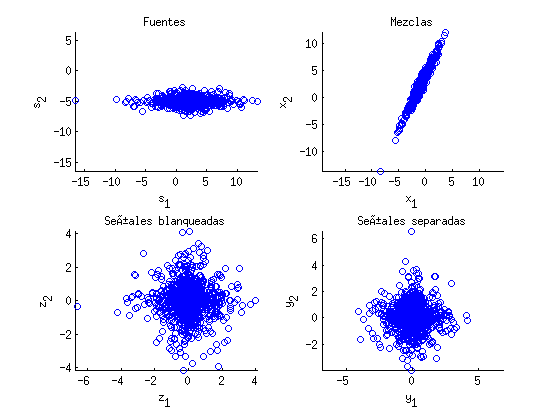
\includegraphics [width=\textwidth]{Ejercicio4_01.png}
\caption{Señales en cada etapa al aplicar FastICA.}
\label{fig:ejercicio41}
\end{figure}

En la Figura \ref{fig:ejercicio41} se muestra cada una de las etapas requeridas. Las matrices solicitadas se escriben a continuación.

\begin{verbatim}P = [0.00 1.00],	 D = [0.85 -0.14]
    [1.00 0.00],	     [-0.44 -0.35]
\end{verbatim}

\begin{verbatim}
% Comparación entre señales separadas y fuentes
figure
subplot(2,2,1)
plot(s{1}(1:60)); ylim([-10, 10]);
ylabel('s_1')

subplot(2,2,2)
plot(s{2}(1:60)); ylim([-10, 10]);
ylabel('s_2');

subplot(2,2,3)
plot(Y(1,1:60)); ylim([-10, 10]);
ylabel('y_1');

subplot(2,2,4)
plot(Y(2,1:60)); ylim([-10, 10]);
ylabel('y_2');
\end{verbatim}

\begin{figure}
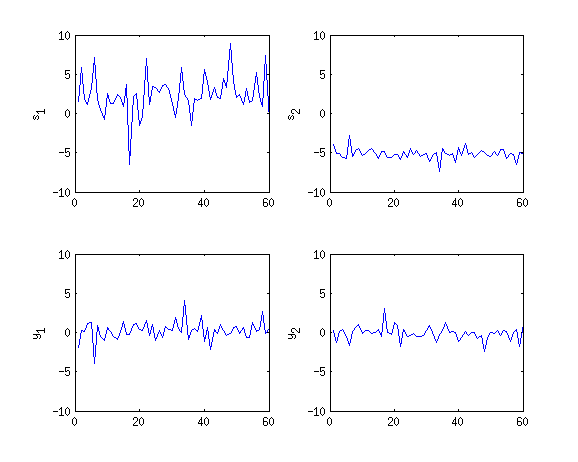
\includegraphics [width=\textwidth]{Ejercicio4_02.png}
\caption{Segmento de las fuentes (arriba) y las señales separadas(abajo). La comparación permite comprobar la matriz $\mathbf{P}$ y $\mathbf{D}$.}
\label{fig:ejercicio41}
\end{figure}


\begin{enumerate}
   \item[c)] ¿La matriz de separación $\mathbf{W}$ es la inversa de la matriz de mezcla $\mathbf{A}$ utilizada?
\end{enumerate}

No lo es, en el caso ideal lo sería. En la práctica se espera obtener $\mathbf{P} \mathbf{D} = \mathbf{W}^T\mathbf{A}$, donde $\mathbf{P}$ es una matriz de permutación y \ensuremath{\backslash}mathbf\{D\} es una matriz de escalado (también involucra el signo para invertir la señal de ser necesario).

\begin{enumerate}

   \item[d)]  ¿Cómo se afecta este resultado si agrega una componente de ruido gaussiano al modelo generativo?
\end{enumerate}

La base del funcionamiento de ICA está en maximizar la lejanía de las distribuciones de cada señal recuperada de la distribución gaussiana. Si el ruido gaussiano tiene una potencia importante en relación a las fuentes es de esperar que no se logren recuperar. Si el ruido no enmascara por demás las fuentes es posible recuperar las fuentes.

\begin{enumerate}

   \item[e)]  ¿Qué ocurre si una de las fuentes es gaussiana? ¿Y si ambas lo son?
\end{enumerate}

Si una de las fuentes es gaussiana todavía es posible encontrar las fuentes, si las dos lo son no es posible.


\end{document}